\Subsubsubsection{Potencia}

Para la unidad de potencia se utilizarán paneles solares y una batería de gel de ciclo profundo conectados a la placa DFR0580, la cual se ocupa de cargar la batería. De esta se obtienen 4 salidas de tensión:
\begin{itemize}
	\item Dos salidas de 5 V y 2.5 A [USB].
	\item Una salida de 5 V y 5 A.
	\item Una salida de 12 V y 8 A.
\end{itemize}

Con estas salidas se alimentarán todos los módulos, a excepción del oscilador de potencia, ya que esta necesita una etapa DC-DC para así la cual eleva la tensión. Para ello se emplea una fuente switching de topología Boost.

\Subsubsubsection{Sensado}

En esta sección, se hablará del conexionado de los sensores.
Para esto se diseño una placa de soporte para la raspberry pi, a modo de shield, donde se haya el módulo RTC y el acondicionamiento para los sensores de humedad, temperatura, luminosidad y presencia. También el lugar de conexión de la cámara y abastecimiento de energía.\\
Se desarrollo una placa del tipo shield para la raspberry pi como adición para el módulo RTC cuya comunicación se relaiza por el bus I2C, ademas se raliza el acondicionamiento para las señales de los sensores. La placa de sensores utiliza el bus I2C, alimentación de 3.3V, la referencia de tierra y un pin GPIO para comunicación serial.\\
Cabe mencionar que el conexionado con el sensor de luminosidad y RTC se utilizará el protocolo de comunicación $I^2C$ en modo multi-slave.

\begin{figure}[H]
	\centering
	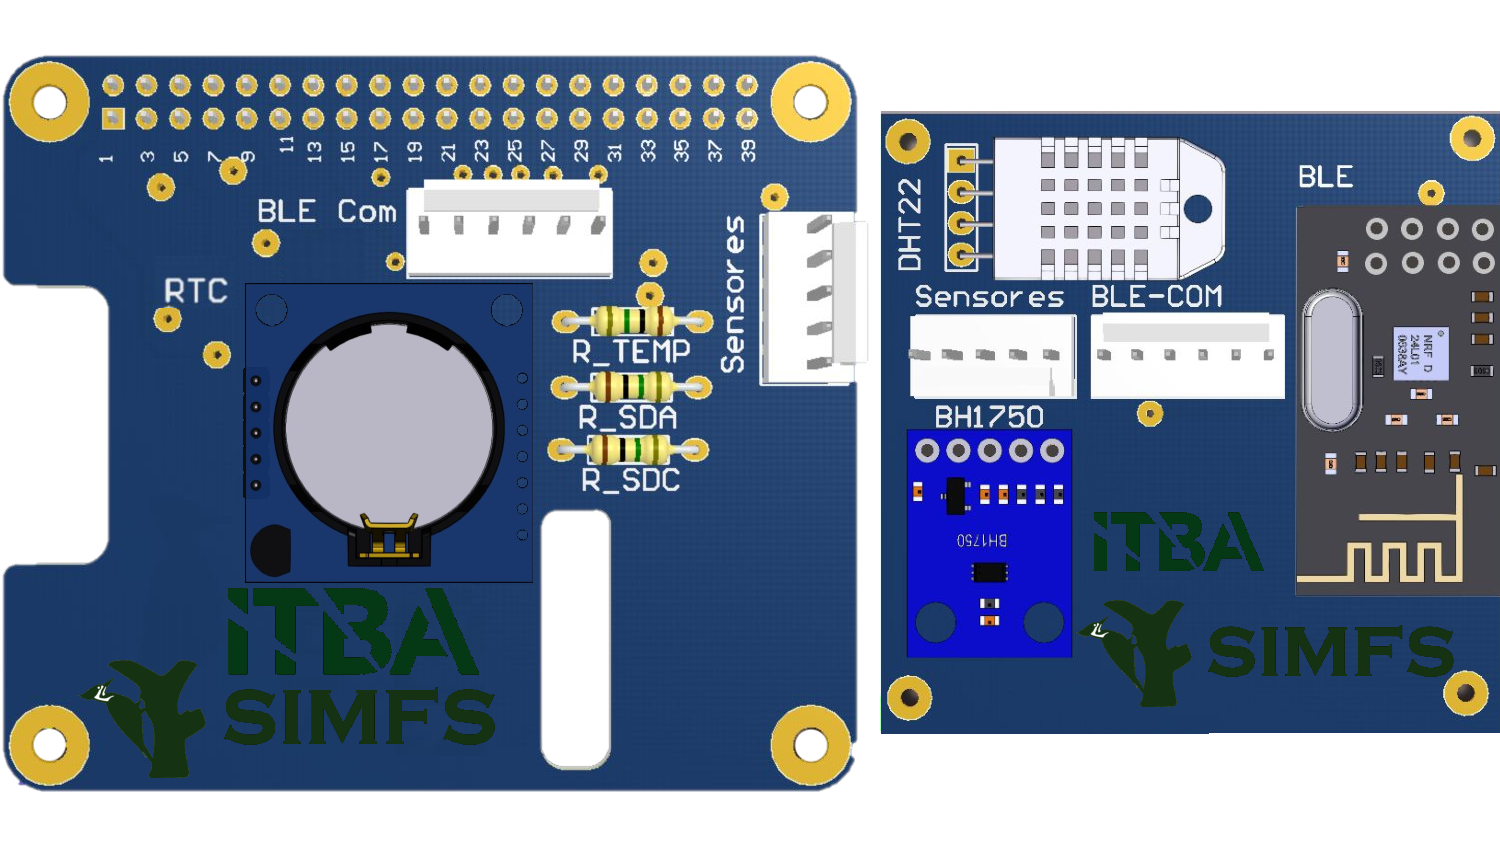
\includegraphics[width=0.9\linewidth,page=1]{ImagenesIngenieria de Detalle/RPI}		
	\caption{Shield raspberry pi.}
	\label{fig:conexionado_Rpi}
\end{figure}

En la placa de sensores se observa que el pin serial GPIO corresponde a la comunicación del sensor de temperatura y humedad DHT-22, y el bus I2C al sensor de luminosidad BH-1750, finalmente cuenta con un conector exclusivo para la comunicación del sensor de presencia.

La raspberry pi cuenta con un conector destinado al uso de una cámara el cual se muestra en la figura (\ref{fig:rpiFront})
\begin{figure}[H]
	\centering
	\includegraphics[width=\linewidth,page=3]{ImagenesIngenieria de Detalle/RPI}		
	\caption{Conexionado cámara.}
	\label{fig:rpiFront}
\end{figure}
Además cuenta con un slot para una tarjeta SD la cual puede ser usada no solo para la imagen de sistema sino que de almacenamiento.
\begin{figure}[H]
	\centering
	\includegraphics[width=0.9\linewidth,page=2]{ImagenesIngenieria de Detalle/RPI}		
	\caption{Conexionado tarjeta SD.}
	\label{fig:rpiBack}
\end{figure}

